\documentclass{standalone}
\usepackage{tikz}
\usetikzlibrary{patterns, positioning}

\begin{document}
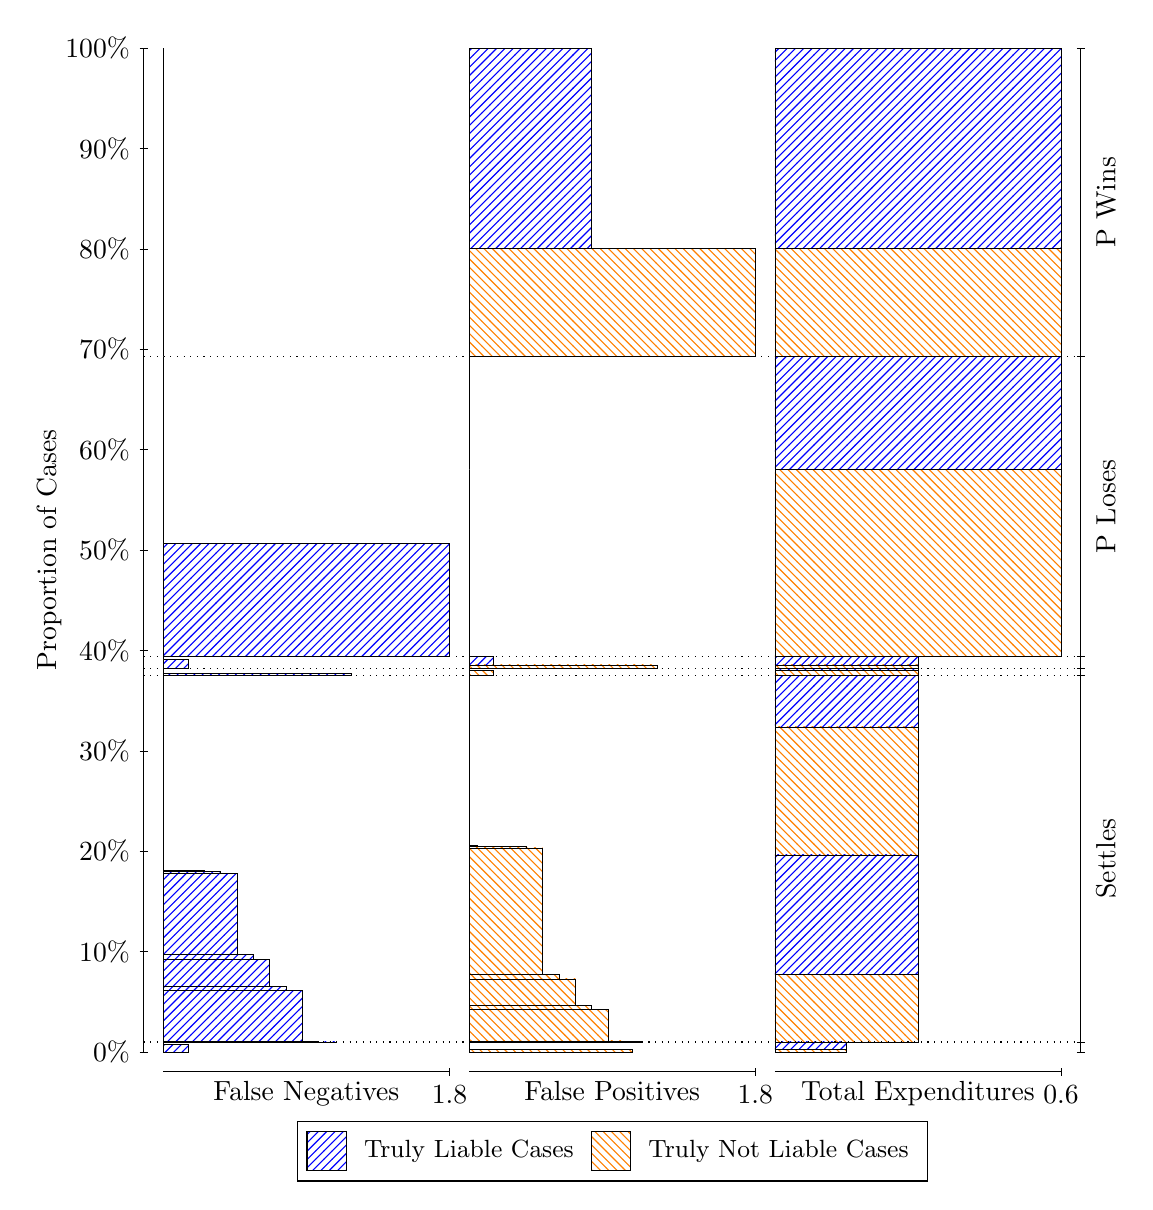
\begin{tikzpicture}
\draw[black, very thin] (1.5,1.75) -- (1.5,14.5);
\node[rotate=90, anchor=center] at (0.3, 8.125) {Proportion of Cases};
\draw[black, very thin] (1.45,1.75) -- (1.55,1.75);
\node[anchor=east] at (1.45, 1.75) {0\%};
\draw[black, very thin] (1.45,3.025) -- (1.55,3.025);
\node[anchor=east] at (1.45, 3.025) {10\%};
\draw[black, very thin] (1.45,4.3) -- (1.55,4.3);
\node[anchor=east] at (1.45, 4.3) {20\%};
\draw[black, very thin] (1.45,5.575) -- (1.55,5.575);
\node[anchor=east] at (1.45, 5.575) {30\%};
\draw[black, very thin] (1.45,6.85) -- (1.55,6.85);
\node[anchor=east] at (1.45, 6.85) {40\%};
\draw[black, very thin] (1.45,8.125) -- (1.55,8.125);
\node[anchor=east] at (1.45, 8.125) {50\%};
\draw[black, very thin] (1.45,9.4) -- (1.55,9.4);
\node[anchor=east] at (1.45, 9.4) {60\%};
\draw[black, very thin] (1.45,10.675) -- (1.55,10.675);
\node[anchor=east] at (1.45, 10.675) {70\%};
\draw[black, very thin] (1.45,11.95) -- (1.55,11.95);
\node[anchor=east] at (1.45, 11.95) {80\%};
\draw[black, very thin] (1.45,13.225) -- (1.55,13.225);
\node[anchor=east] at (1.45, 13.225) {90\%};
\draw[black, very thin] (1.45,14.5) -- (1.55,14.5);
\node[anchor=east] at (1.45, 14.5) {100\%};

\draw[black, very thin] (13.4,1.75) -- (13.4,14.5);
\draw[black, very thin] (13.35,1.75) -- (13.45,1.75);
\node[anchor=west] at (13.35, 1.75) {};
\draw[black, very thin] (13.35,1.8773) -- (13.45,1.8773);
\node[anchor=west] at (13.35, 1.8773) {};
\draw[black, very thin] (13.35,6.5361) -- (13.45,6.5361);
\node[anchor=west] at (13.35, 6.5361) {};
\draw[black, very thin] (13.35,6.624) -- (13.45,6.624);
\node[anchor=west] at (13.35, 6.624) {};
\draw[black, very thin] (13.35,6.7761) -- (13.45,6.7761);
\node[anchor=west] at (13.35, 6.7761) {};
\draw[black, very thin] (13.35,10.581) -- (13.45,10.581);
\node[anchor=west] at (13.35, 10.581) {};
\draw[black, very thin] (13.35,14.5) -- (13.45,14.5);
\node[anchor=west] at (13.35, 14.5) {};

\draw[black, very thin, pattern color=blue, pattern=north east lines] (1.75,1.75) rectangle (2.0614,1.8423);
\draw[black, very thin, pattern color=orange, pattern=north west lines] (1.75,1.8423) rectangle (1.75,1.8773);
\draw[black, very thin, pattern color=blue, pattern=north east lines] (1.75,1.8773) rectangle (3.93,1.8787);
\draw[black, very thin, pattern color=blue, pattern=north east lines] (1.75,1.8787) rectangle (3.7224,1.8842);
\draw[black, very thin, pattern color=blue, pattern=north east lines] (1.75,1.8842) rectangle (3.5148,2.5347);
\draw[black, very thin, pattern color=blue, pattern=north east lines] (1.75,2.5347) rectangle (3.3071,2.5877);
\draw[black, very thin, pattern color=blue, pattern=north east lines] (1.75,2.5877) rectangle (3.0995,2.928);
\draw[black, very thin, pattern color=blue, pattern=north east lines] (1.75,2.928) rectangle (2.8919,2.9849);
\draw[black, very thin, pattern color=blue, pattern=north east lines] (1.75,2.9849) rectangle (2.6843,4.0132);
\draw[black, very thin, pattern color=blue, pattern=north east lines] (1.75,4.0132) rectangle (2.4767,4.0386);
\draw[black, very thin, pattern color=blue, pattern=north east lines] (1.75,4.0386) rectangle (2.269,4.0517);
\draw[black, very thin, pattern color=orange, pattern=north west lines] (1.75,4.0517) rectangle (1.75,6.5361);
\draw[black, very thin, pattern color=blue, pattern=north east lines] (1.75,6.5361) rectangle (4.1376,6.5606);
\draw[black, very thin, pattern color=orange, pattern=north west lines] (1.75,6.5606) rectangle (1.75,6.624);
\draw[black, very thin, pattern color=blue, pattern=north east lines] (1.75,6.624) rectangle (2.0614,6.7349);
\draw[black, very thin, pattern color=orange, pattern=north west lines] (1.75,6.7349) rectangle (1.75,6.7761);
\draw[black, very thin, pattern color=blue, pattern=north east lines] (1.75,6.7761) rectangle (5.3833,8.2093);
\draw[black, very thin, pattern color=orange, pattern=north west lines] (1.75,8.2093) rectangle (1.75,10.581);
\draw[black, very thin, pattern color=orange, pattern=north west lines] (1.75,10.581) rectangle (1.75,11.96);
\draw[black, very thin, pattern color=blue, pattern=north east lines] (1.75,11.96) rectangle (1.75,14.5);
\draw[black, very thin, pattern color=orange, pattern=north west lines] (5.6333,1.75) rectangle (7.7095,1.7849);
\draw[black, very thin, pattern color=blue, pattern=north east lines] (5.6333,1.7849) rectangle (5.6333,1.8773);
\draw[black, very thin, pattern color=orange, pattern=north west lines] (5.6333,1.8773) rectangle (7.8133,1.8813);
\draw[black, very thin, pattern color=orange, pattern=north west lines] (5.6333,1.8813) rectangle (7.6057,1.8899);
\draw[black, very thin, pattern color=orange, pattern=north west lines] (5.6333,1.8899) rectangle (7.3981,2.2915);
\draw[black, very thin, pattern color=orange, pattern=north west lines] (5.6333,2.2915) rectangle (7.1905,2.3371);
\draw[black, very thin, pattern color=orange, pattern=north west lines] (5.6333,2.3371) rectangle (6.9829,2.677);
\draw[black, very thin, pattern color=orange, pattern=north west lines] (5.6333,2.677) rectangle (6.7752,2.733);
\draw[black, very thin, pattern color=orange, pattern=north west lines] (5.6333,2.733) rectangle (6.7752,2.7361);
\draw[black, very thin, pattern color=orange, pattern=north west lines] (5.6333,2.7361) rectangle (6.5676,4.3426);
\draw[black, very thin, pattern color=orange, pattern=north west lines] (5.6333,4.3426) rectangle (6.36,4.3575);
\draw[black, very thin, pattern color=orange, pattern=north west lines] (5.6333,4.3575) rectangle (6.1524,4.3617);
\draw[black, very thin, pattern color=blue, pattern=north east lines] (5.6333,4.3617) rectangle (5.7371,4.3748);
\draw[black, very thin, pattern color=blue, pattern=north east lines] (5.6333,4.3748) rectangle (5.6333,6.5361);
\draw[black, very thin, pattern color=orange, pattern=north west lines] (5.6333,6.5361) rectangle (5.9448,6.5995);
\draw[black, very thin, pattern color=blue, pattern=north east lines] (5.6333,6.5995) rectangle (5.6333,6.624);
\draw[black, very thin, pattern color=orange, pattern=north west lines] (5.6333,6.624) rectangle (8.021,6.6651);
\draw[black, very thin, pattern color=blue, pattern=north east lines] (5.6333,6.6651) rectangle (5.9448,6.7761);
\draw[black, very thin, pattern color=orange, pattern=north west lines] (5.6333,6.7761) rectangle (5.6333,9.1482);
\draw[black, very thin, pattern color=blue, pattern=north east lines] (5.6333,9.1482) rectangle (5.6333,10.581);
\draw[black, very thin, pattern color=orange, pattern=north west lines] (5.6333,10.581) rectangle (9.2667,11.96);
\draw[black, very thin, pattern color=blue, pattern=north east lines] (5.6333,11.96) rectangle (7.1905,14.5);
\draw[black, very thin, pattern color=orange, pattern=north west lines] (9.5167,1.75) rectangle (10.425,1.7849);
\draw[black, very thin, pattern color=blue, pattern=north east lines] (9.5167,1.7849) rectangle (10.425,1.8773);
\draw[black, very thin, pattern color=orange, pattern=north west lines] (9.5167,1.8773) rectangle (11.333,2.733);
\draw[black, very thin, pattern color=blue, pattern=north east lines] (9.5167,2.733) rectangle (11.333,4.2472);
\draw[black, very thin, pattern color=orange, pattern=north west lines] (9.5167,4.2472) rectangle (11.333,4.2515);
\draw[black, very thin, pattern color=blue, pattern=north east lines] (9.5167,4.2515) rectangle (11.333,4.2529);
\draw[black, very thin, pattern color=orange, pattern=north west lines] (9.5167,4.2529) rectangle (11.333,5.8774);
\draw[black, very thin, pattern color=blue, pattern=north east lines] (9.5167,5.8774) rectangle (11.333,6.5361);
\draw[black, very thin, pattern color=orange, pattern=north west lines] (9.5167,6.5361) rectangle (11.333,6.5995);
\draw[black, very thin, pattern color=blue, pattern=north east lines] (9.5167,6.5995) rectangle (11.333,6.624);
\draw[black, very thin, pattern color=orange, pattern=north west lines] (9.5167,6.624) rectangle (11.333,6.6651);
\draw[black, very thin, pattern color=blue, pattern=north east lines] (9.5167,6.6651) rectangle (11.333,6.7761);
\draw[black, very thin, pattern color=orange, pattern=north west lines] (9.5167,6.7761) rectangle (13.15,9.1482);
\draw[black, very thin, pattern color=blue, pattern=north east lines] (9.5167,9.1482) rectangle (13.15,10.581);
\draw[black, very thin, pattern color=orange, pattern=north west lines] (9.5167,10.581) rectangle (13.15,11.96);
\draw[black, very thin, pattern color=blue, pattern=north east lines] (9.5167,11.96) rectangle (13.15,14.5);
\draw[black, dotted] (1.5,1.8773) -- (13.4,1.8773);
\draw[black, dotted] (1.5,6.5361) -- (13.4,6.5361);
\draw[black, dotted] (1.5,6.624) -- (13.4,6.624);
\draw[black, dotted] (1.5,6.7761) -- (13.4,6.7761);
\draw[black, dotted] (1.5,10.581) -- (13.4,10.581);
\draw[black, very thin] (1.75,1.5) -- (5.3833,1.5);
\node[anchor=north] at (3.5667, 1.5) {False Negatives};
\draw[black, very thin] (5.3833,1.45) -- (5.3833,1.55);
\node[anchor=north] at (5.3833, 1.45) {1.8};

\draw[black, very thin] (5.6333,1.5) -- (9.2667,1.5);
\node[anchor=north] at (7.45, 1.5) {False Positives};
\draw[black, very thin] (9.2667,1.45) -- (9.2667,1.55);
\node[anchor=north] at (9.2667, 1.45) {1.8};

\draw[black, very thin] (9.5167,1.5) -- (13.15,1.5);
\node[anchor=north] at (11.333, 1.5) {Total Expenditures};
\draw[black, very thin] (13.15,1.45) -- (13.15,1.55);
\node[anchor=north] at (13.15, 1.45) {0.6};


\node[black, centered, rotate=90] at (13.72, 4.2067) {Settles};


\node[black, centered, rotate=90] at (13.72, 8.6788) {P Loses};
\node[black, centered, rotate=90] at (13.72, 12.541) {P Wins};

\draw (7.449999999999999,1.5) node[draw=none] (baseCoordinate) {};
\begin{scope}[align=center]
        \matrix[scale=0.5, draw=black, below=0.5cm of baseCoordinate, nodes={draw}, column sep=0.1cm]{
            \node[rectangle, draw, minimum width=0.5cm, minimum height=0.5cm, pattern=north east lines, pattern color=blue] {}; &
            \node[draw=none, font=\small] (B) {Truly Liable Cases}; &
            \node[rectangle, draw, minimum width=0.5cm, minimum height=0.5cm, pattern=north west lines, pattern color=orange] {}; &
            \node[draw=none, font=\small] (B) {Truly Not Liable Cases}; \\
            };
\end{scope}

\end{tikzpicture}
\end{document}